\chapter{Design Methodology}
Define specs; select architecture; perform small-signal and large-signal simulations; run PSS/Pnoise or time-domain jitter; tune \(K_{VCO}\); linearize tuning; validate across PVT; finalize layout.

\section{Meta-Heuristic Optimization (Bonus)}
Apply a simple GA/PSO to choose \(L\), varactor bank size, and bias to minimize a cost combining PN@offsets, power, and tuning coverage. The flow evaluates a fast surrogate (analytical + corner multipliers) and verifies finalists with detailed simulations. Convergence typically occurs in tens of iterations; constraints enforce KVCO and range.

\begin{figure}[H]
  \centering
  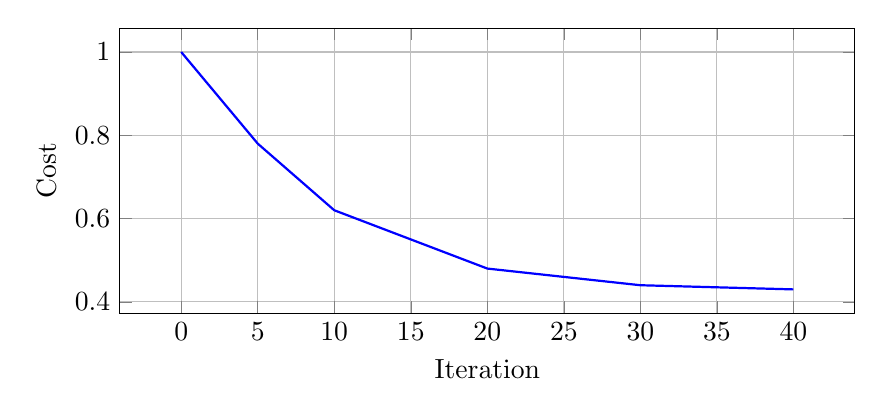
\begin{tikzpicture}
    \begin{axis}[width=0.9\linewidth, height=5.2cm, xlabel={Iteration}, ylabel={Cost}, grid=both]
      \addplot[blue, thick] table[row sep=\\]{x y \\
        0  1.00 \\
        5  0.78 \\
        10 0.62 \\
        20 0.48 \\
        30 0.44 \\
        40 0.43 \\
      };
    \end{axis}
  \end{tikzpicture}
  \caption{Illustrative convergence of a meta-heuristic cost function}
\end{figure}

\section{Step-by-Step Flow}
\begin{enumerate}
  \item Requirements: define PN mask, tuning range, power, spur limits, area.
  \item Architecture choice: ring vs LC; select $L$/$Q$ plan (LC) or stage count (ring).
  \item Initial sizing: set swing, estimate $K_{VCO}$; plan coarse/fine banks and overlap.
  \item Simulation loop: PSS/Pnoise and transient noise; sweep bias and device widths.
  \item Optimization (optional): run GA/PSO on surrogate; verify winners with EM/parasitic.
  \item PVT/Monte Carlo: confirm startup margin, PN spread, spur sensitivity.
  \item Layout and PDN: symmetric routing, guard rings, decoupling networks.
  \item Final validation: measurement hooks, buffer levels, documentation.
\end{enumerate}

\section{Deliverables}
\begin{itemize}
  \item Report with specs, models, results, and comparisons.
  \item Simulation decks and scripts (transient noise, PSS/Pnoise, sweep).
  \item Optional: Python/OCN code for meta-heuristic optimization and data export.
\end{itemize}

\section{Optimization Criteria Matrix}
We combine the main figures of merit (FOMs) in a weighted cost. Typical weights prioritize phase noise while keeping power and range within constraints.
\begin{table}[H]
  \centering
  \begin{tabular}{llll}
    \toprule
    Criterion & Symbol & Target/Constraint & Weight \\
    \midrule
    PN@100 kHz (dBc/Hz) & $\mathcal{L}_{100k}$ & $< -100$ & 0.5 \\
    Power (mW) & $P$ & $< 10$ & 0.2 \\
    Range (\%) & $R$ & $\ge 40$ & 0.2 \\
    $K_{VCO}$ (MHz/V) & $K$ & 1–3 & 0.1 \\
    \bottomrule
  \end{tabular}
  \caption{Example multi-objective weights for meta-heuristic cost}
\end{table}

\section{Optimization Pipeline}
\begin{figure}[H]
  \centering
  \begin{tikzpicture}[node distance=1.6cm, >=Latex]
    \tikzstyle{blk}=[draw, rounded corners, minimum width=3.0cm, minimum height=0.9cm]
    \node[blk] (specs) {Specs \& Constraints};
    \node[blk, right=of specs] (sur) {Surrogate Model};
    \node[blk, right=of sur] (ga) {GA/PSO Search};
    \node[blk, right=of ga] (verify) {Detailed Sims (PSS/Pnoise, EM)};
    \node[blk, right=of verify] (pvt) {PVT/MC Sweep};
    \node[blk, right=of pvt] (final) {Finalize & Handoff};
    \draw[->] (specs) -- (sur);
    \draw[->] (sur) -- (ga);
    \draw[->] (ga) -- (verify);
    \draw[->] (verify) -- (pvt);
    \draw[->] (pvt) -- (final);
  \end{tikzpicture}
  \caption{Optimization pipeline from specs to final validated design}
\end{figure}


\section{Requirements to Numbers}
Translate verbal requirements into quantitative targets. For the running example (\SI{10}{\mega\hertz}, $\pm20\%$, \SI{1.8}{\volt}):
\begin{table}[H]
  \centering
  \begin{tabular}{lll}
    \toprule
    Item & Target & Rationale \\
    \midrule
    $f_0$ & \SI{10}{\mega\hertz} & Lab-friendly frequency \\
    Range & $\pm20\%$ & Cover PVT and calibration headroom \\
    $K_{VCO}$ & 1--3 \si{\mega\hertz/\volt} & PLL bandwidth, spur control \\
    PN@100 kHz & $< -100$ dBc/Hz & Low-jitter target \\
    Power & $< \SI{10}{\milli\watt}$ & Portable constraints \\
    Supply & \SI{1.8}{\volt} & Common low-voltage node \\
    \bottomrule
  \end{tabular}
  \caption{Example quantitative targets derived from requirements}
\end{table}

\section{Parameterised Workflow (10 MHz Example)}
\subsection*{1) Architecture Decision}
At \SI{10}{\mega\hertz} with aggressive PN target, choose an LC VCO (higher $Q$) over a ring VCO. If area is extremely constrained and PN relaxed, a ring may be acceptable.

\subsection*{2) Initial Tank Planning}
Pick $L$ from area and $Q$ feasibility. With $L=\SI{100}{\nano H}$:
\[
 C_0 = \frac{1}{(2\pi f_0)^2 L} \approx \SI{2.53}{\pF}
\]
Include parasitics $C_{par}$ and choose varactor span to meet $\pm20\%$.

\subsection*{3) KVCO and Tuning Range}
Select a varactor with slope $\partial C/\partial V$ near mid control. Linearize
\[
 K_{VCO} \approx -\frac{f_0}{2(C_f+C_0)}\,\frac{\partial C}{\partial V}\Big|_{V_{mid}}
\]
Choose $C_f$ to place $K_{VCO}$ in 1--3 \si{\mega Hz/V} window while preserving range.

\subsection*{4) Core and Bias}
Choose complementary cross-coupled pair for symmetry and low flicker upconversion. Size devices for startup margin $\times 2$--$\times 3$ across PVT.

\subsection*{5) Banks and Overlap}
Use a binary coarse bank for range and thermometer fine bank for monotonicity. Ensure fine span bridges adjacent coarse steps over PVT.

\subsection*{6) Simulation Loop}
Run PSS/Pnoise over offsets (1 kHz--10 MHz); sweep bias and device widths. Cross-check time-domain transient-noise jitter and integrate PN to $\sigma_t$.

\subsection*{7) PVT/MC}
Sweep TT/SS/FF, $\pm10\%\,V_{DD}$, $-40$ to $125^\circ$C. Confirm startup margin, range overlap, PN spread, and supply sensitivity.

\subsection*{8) Layout/PDN}
Enforce symmetry, guard rings, triple-well isolation, and close decoupling. Shield high-impedance tank nodes; minimize loop area.

\section{Simulation Recipes}
\subsection*{PSS/Pnoise (Phase Noise)}
\begin{itemize}
  \item Fundamental set to expected $f_0$; allow oscillator to find limit cycle.
  \item Pnoise in jitter or time-averaged mode; enable noise folding; sweep 1 kHz to 10 MHz.
  \item Export $\mathcal{L}(f)$ and integrate to estimate RMS jitter per Chapter~6.
\end{itemize}

\subsection*{Transient Noise (Time-Domain Jitter)}
\begin{itemize}
  \item Enable device noise; simulate multiple milliseconds; capture zero-crossings.
  \item Compute histogram and RMS jitter; compare to integrated PN.
\end{itemize}

\subsection*{Supply Sensitivity and Spurs}
\begin{itemize}
  \item Inject a small sinusoid on $V_{DD}$ at reference-related tones; measure $\Delta f$ and spur levels.
  \item Verify PSRR improvements with tail filtering and local regulation.
\end{itemize}

\section{Common Pitfalls Checklist}
\begin{itemize}
  \item Insufficient startup margin at SS/low-$V_{DD}$/high-$T$ corners.
  \item Fine bank span not bridging adjacent coarse steps across PVT.
  \item Excessive $K_{VCO}$ causing spur sensitivity and loop instability.
  \item Tail current modulation upconverting to phase noise; missing tail filtering.
  \item Layout asymmetry degrading close-in phase noise and KVCO linearity.
\end{itemize}


